\begin{appendices}
    % Appendix titles modifyers
    \renewcommand{\theHchapter}{A\arabic{chapter}}
    \renewcommand{\theHsection}{A\arabic{section}}
    \renewcommand*{\justifyheading}{\raggedleft}
    \titleformat{\chapter}[display]
        {\vspace{-3cm}
            \normalfont\Huge\bfseries\justifyheading}
        {\color{gray} \fontsize{48}{48}\selectfont \appendixname 
        \hspace{0.1cm} \thechapter}
        {20pt}{\fontsize{48}{48}\selectfont}
    \titleformat{\section}
        {\normalfont\Large\bfseries}{\thesection}{1em}{}
    \titleformat{\subsection}
        {\normalfont\large\bfseries}{\thesubsection}{1em}{}
    \chapter{Manual de Usuario}
        En este anexo se facilitará un guía para el usuario. El propósito de esta guía es explicar al usuario cuáles son las capacidades de la aplicación y su modo de uso.
        \section{Registro}
        Para poder utilizar la aplicación el usuario deberá realizar primero el registro en el sistema. Este se realizará pulsando el botón de ``¿No tienes una cuenta? Regístrate'' de la figura
        \begin{figure}[H]
    \centering
    \begin{minipage}{0.3\textwidth}
        \centering
        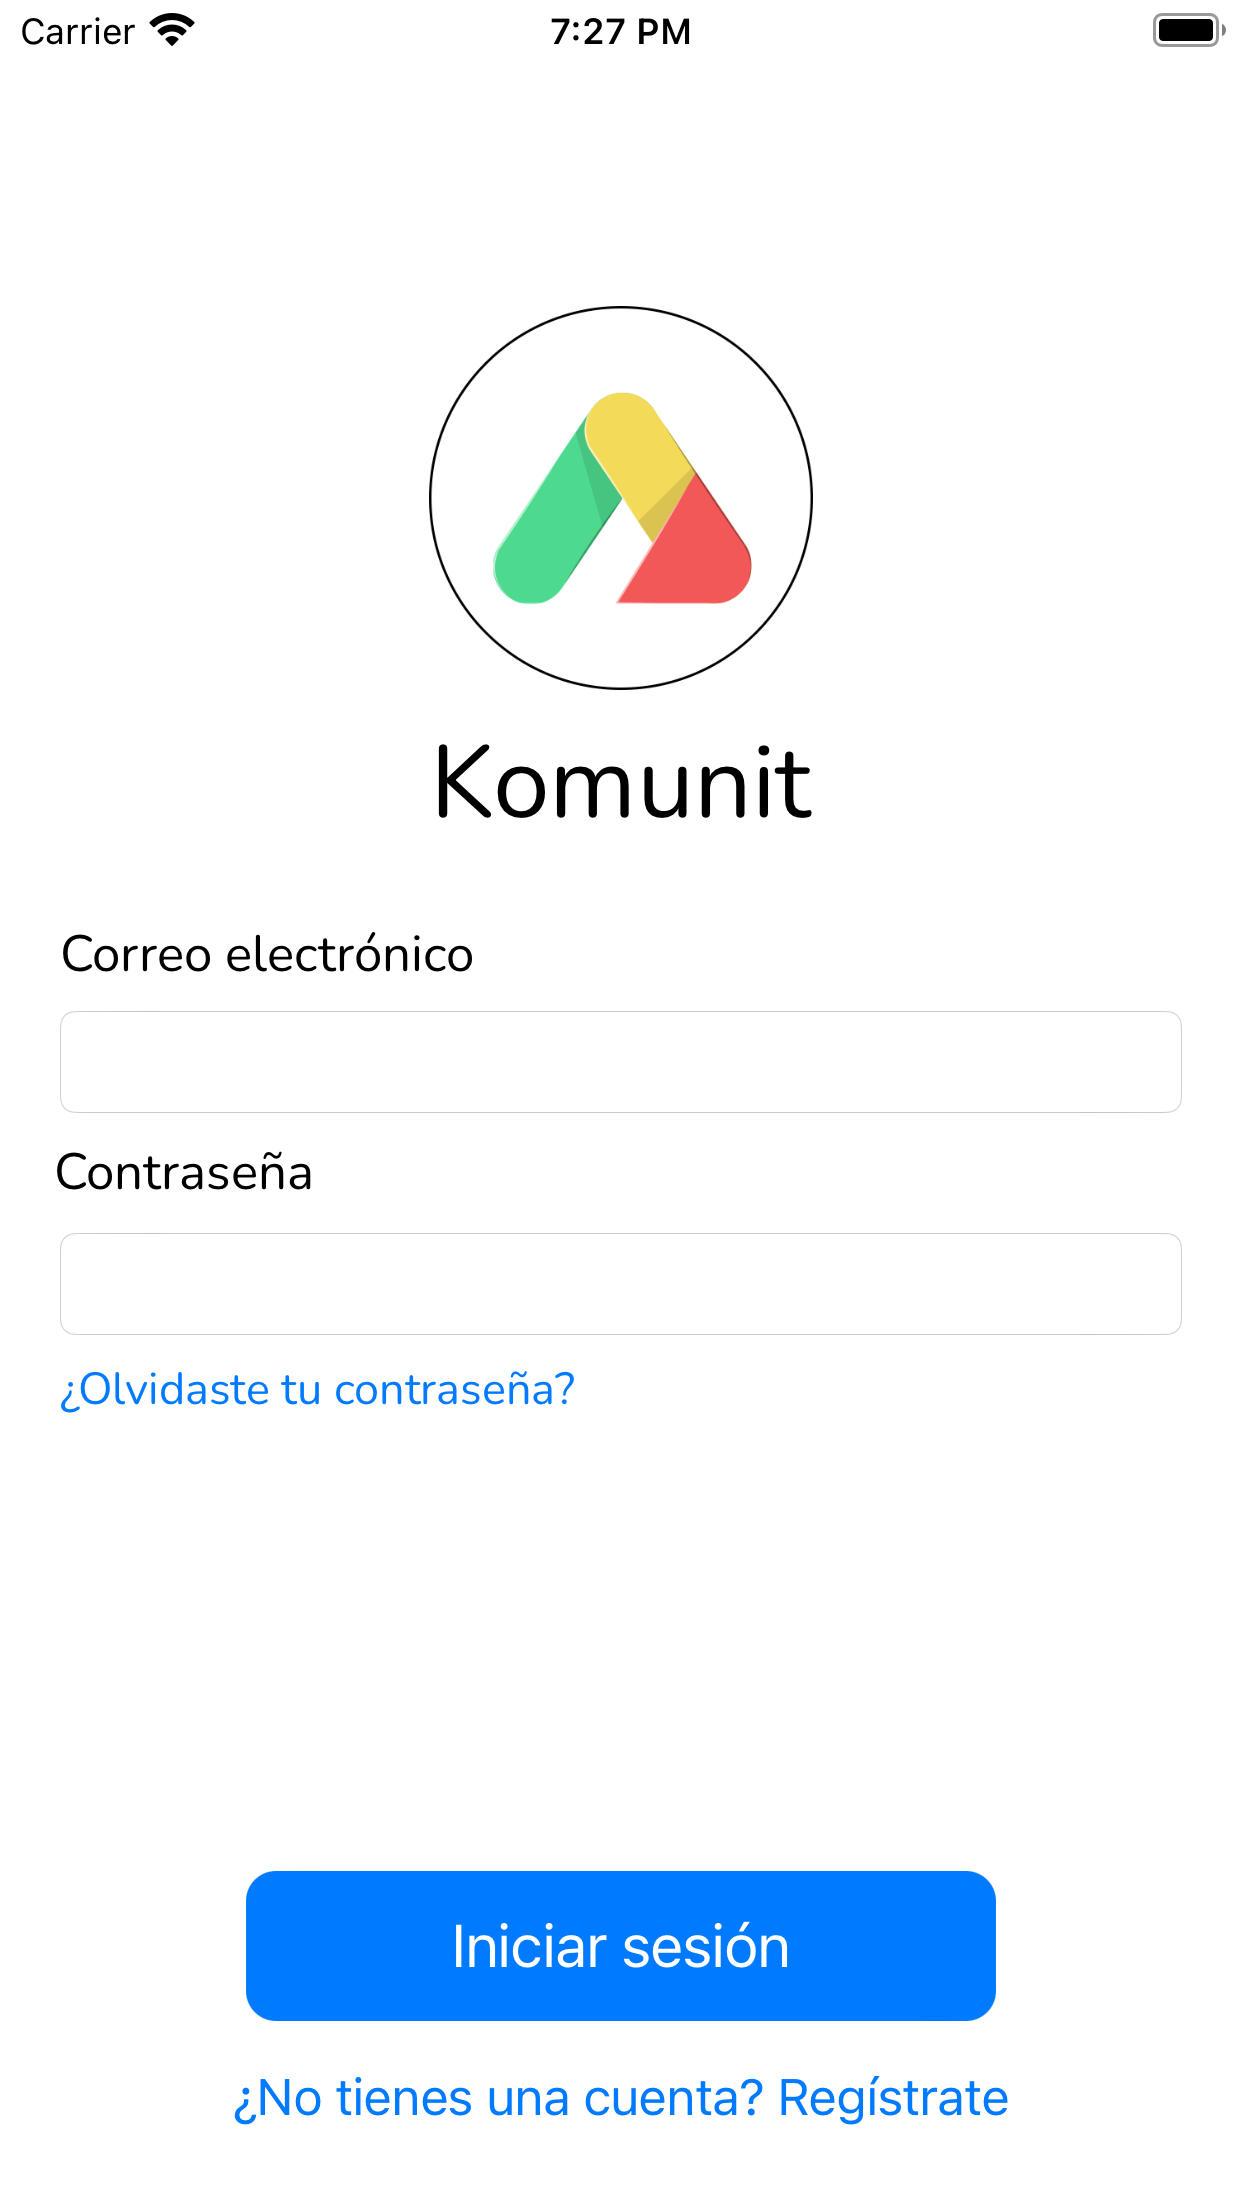
\includegraphics[cframe=black 2pt, width=1\linewidth]{images/manual/login.png}
    \end{minipage}
    \begin{minipage}{0.3\textwidth}
        \centering
        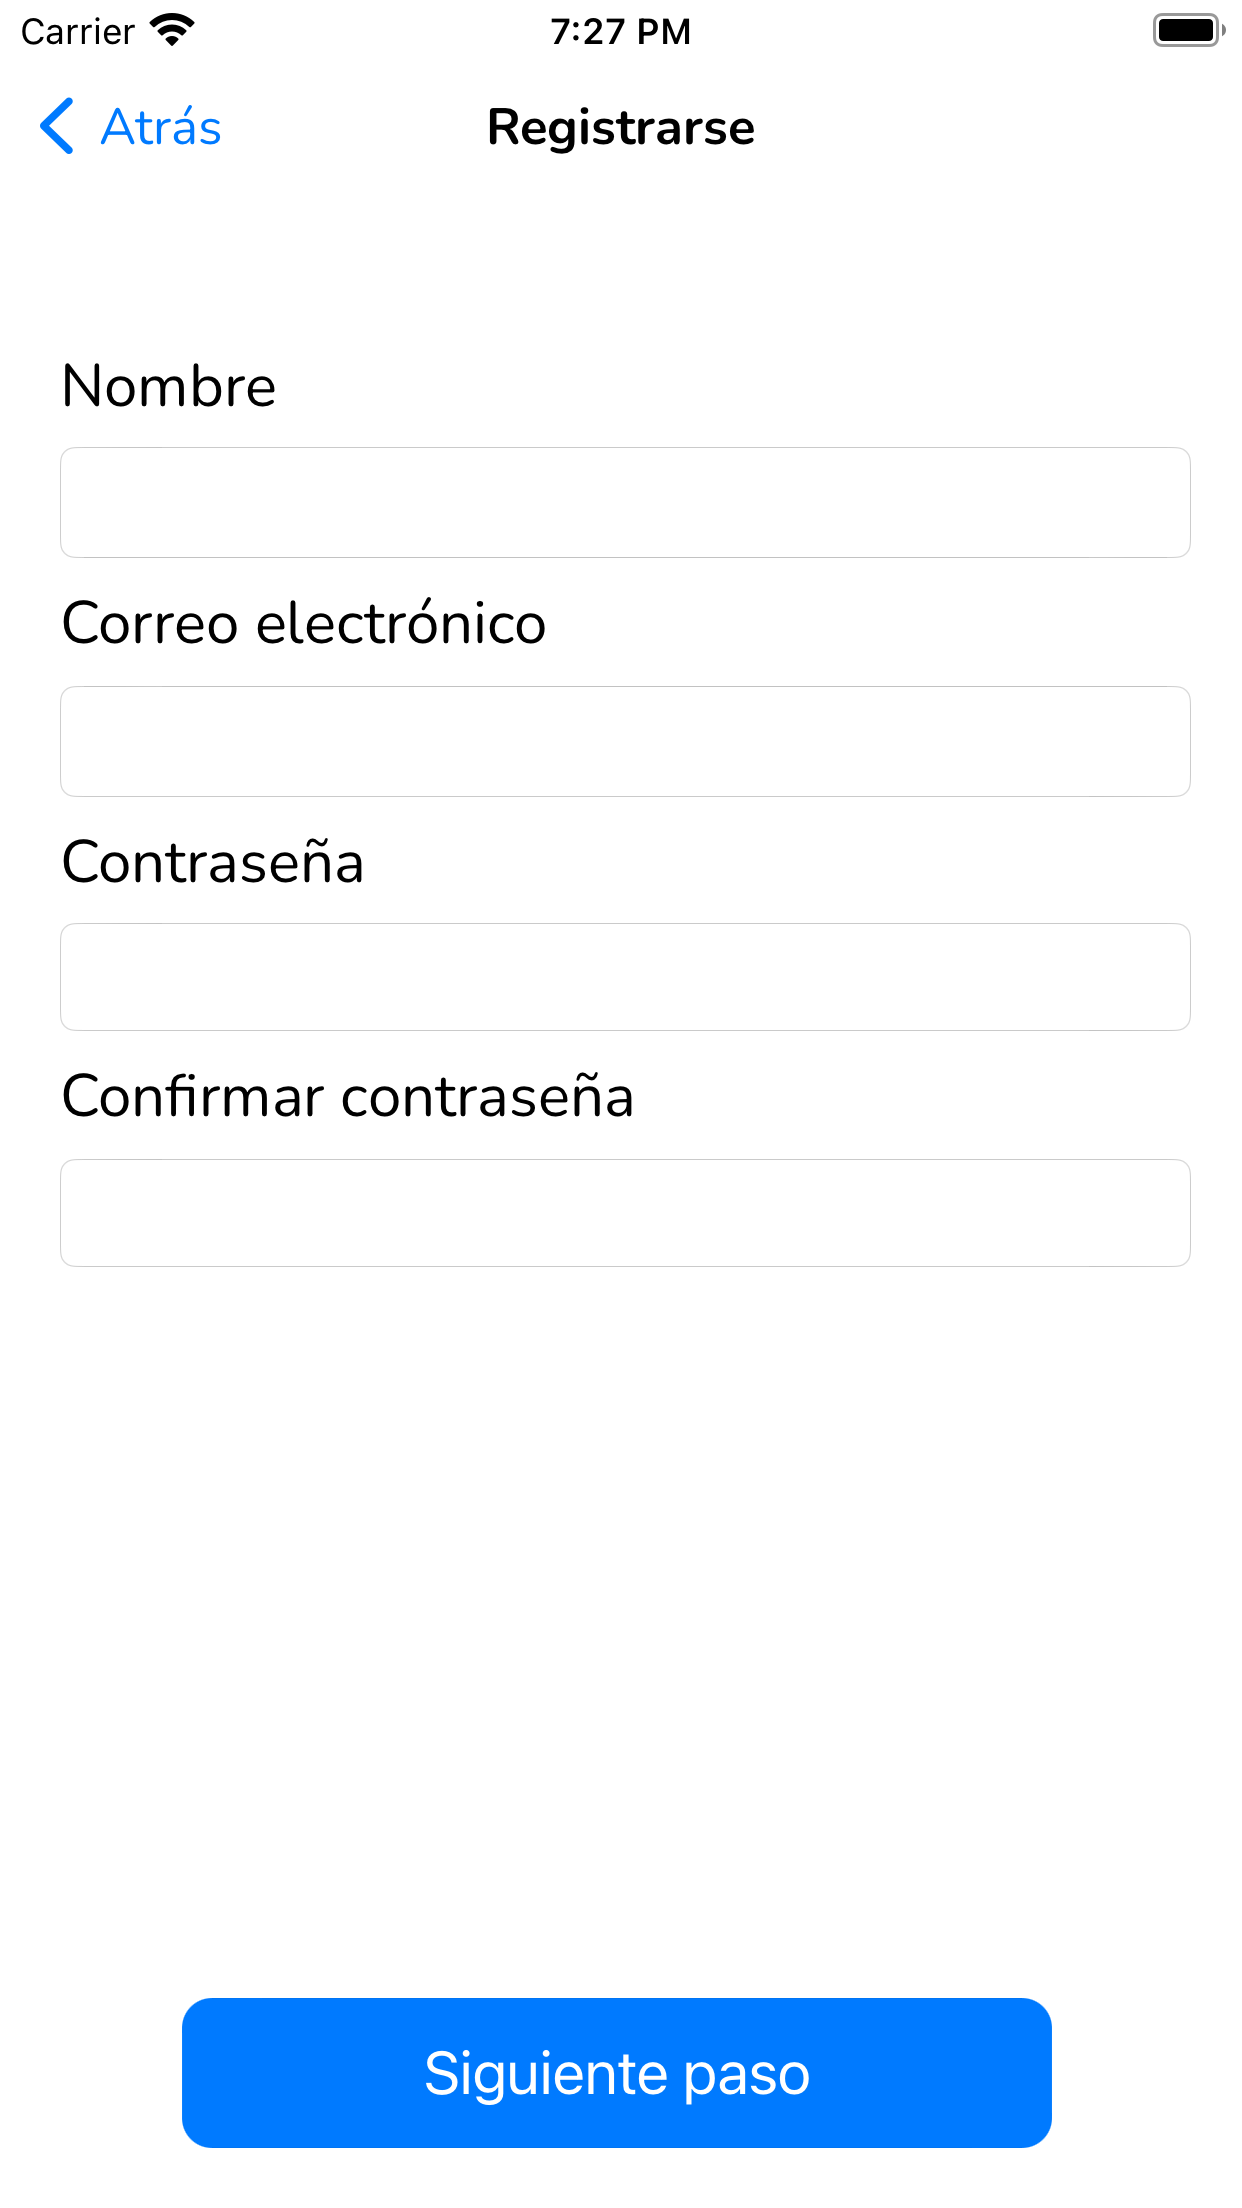
\includegraphics[cframe=black 2pt, width=1\linewidth]{images/manual/registro1.png}
    \end{minipage}
    \begin{minipage}{0.3\textwidth}
        \centering
        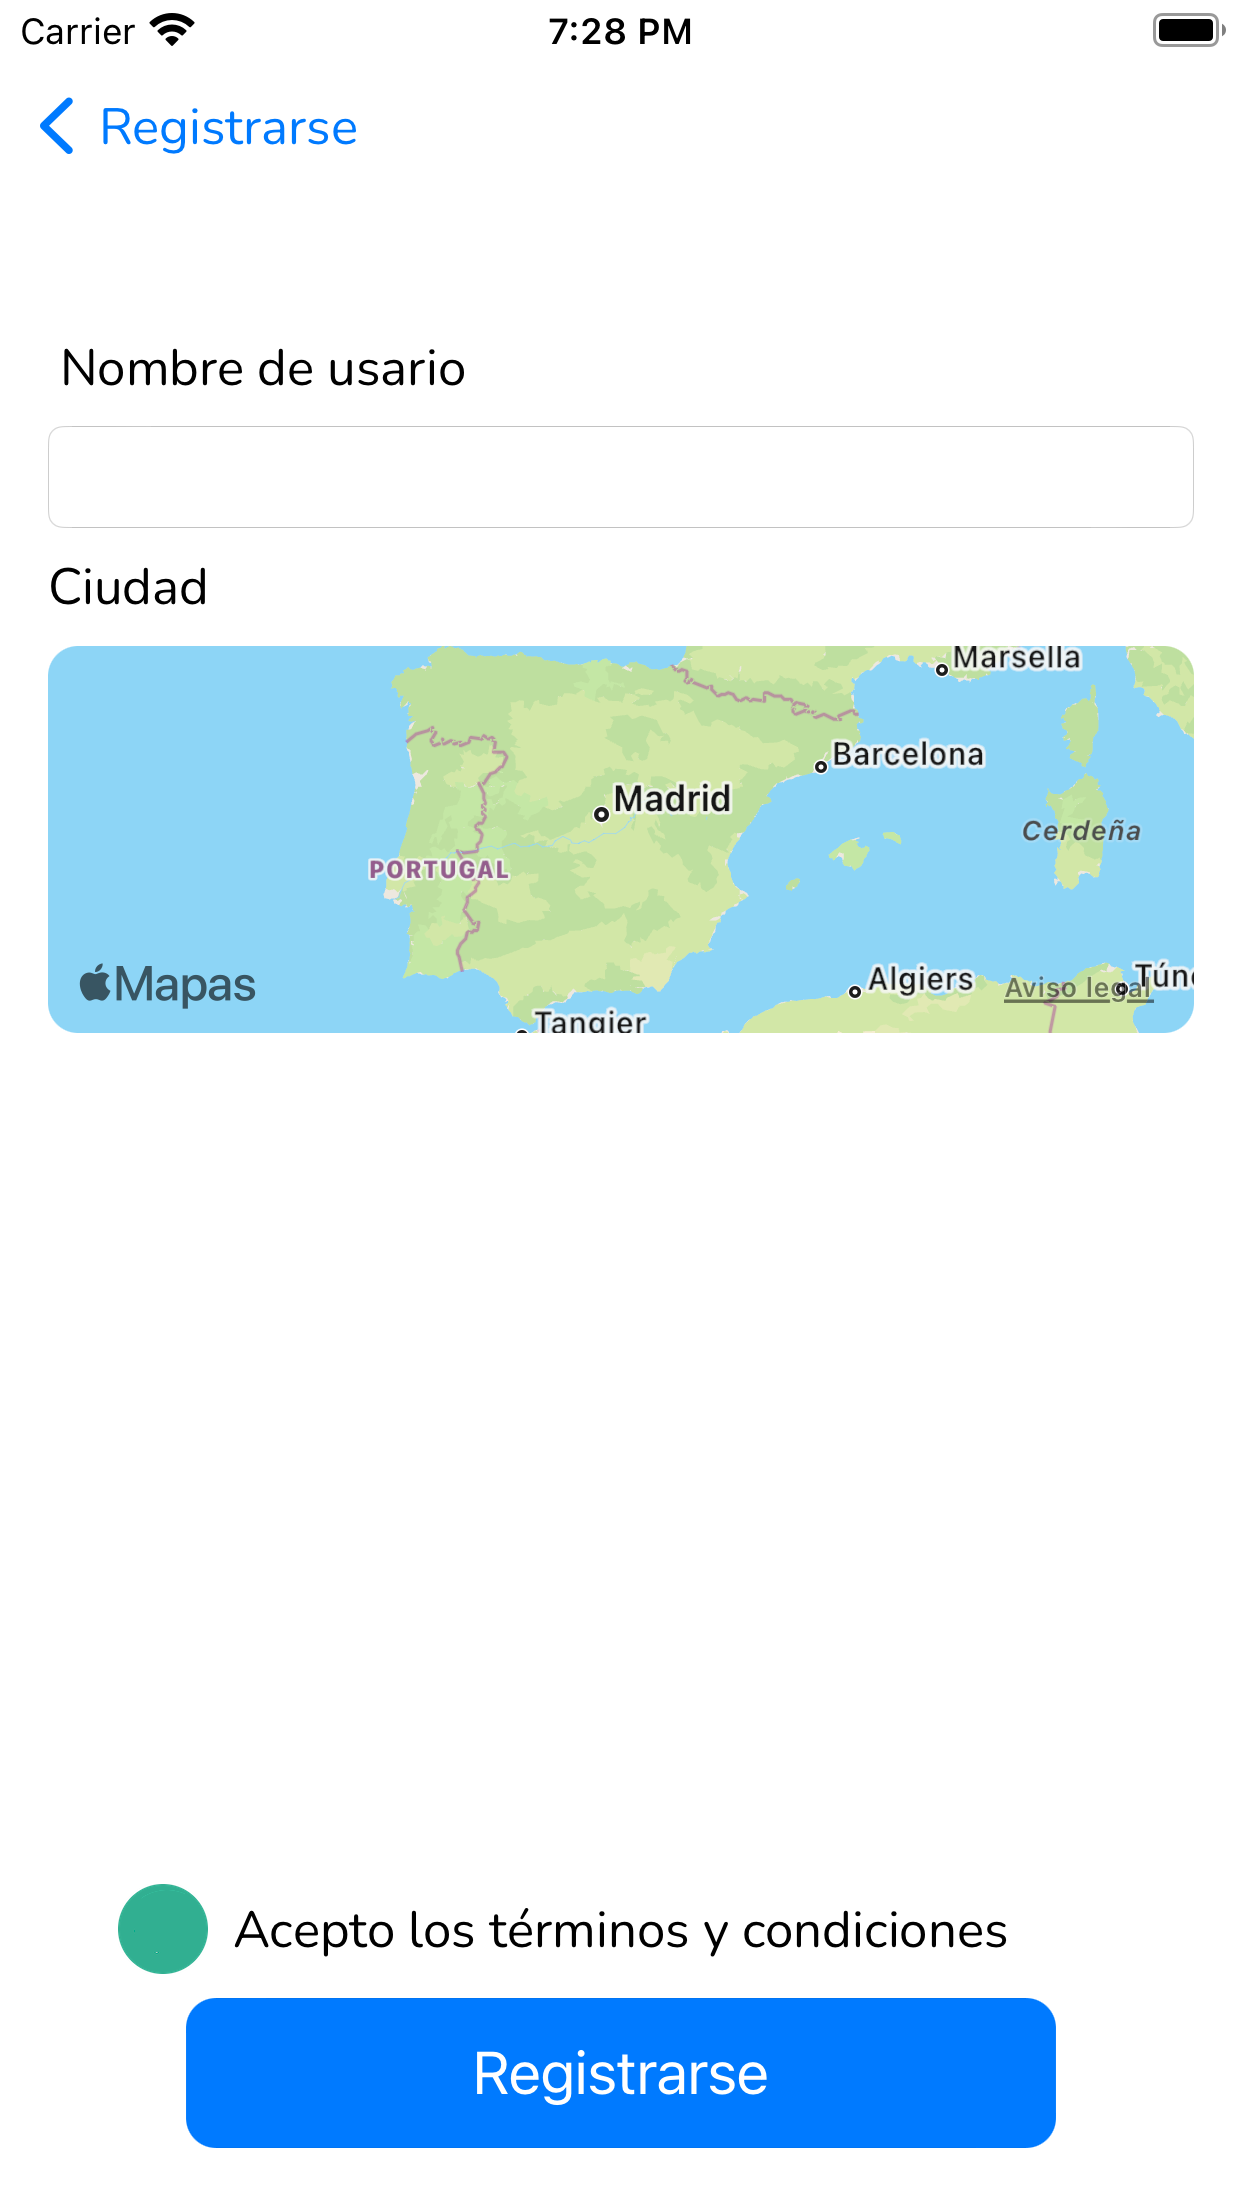
\includegraphics[cframe=black 2pt, width=1\linewidth]{images/manual/registro2.png}
    \end{minipage}
    \begin{minipage}{0.3\textwidth}
        \centering
        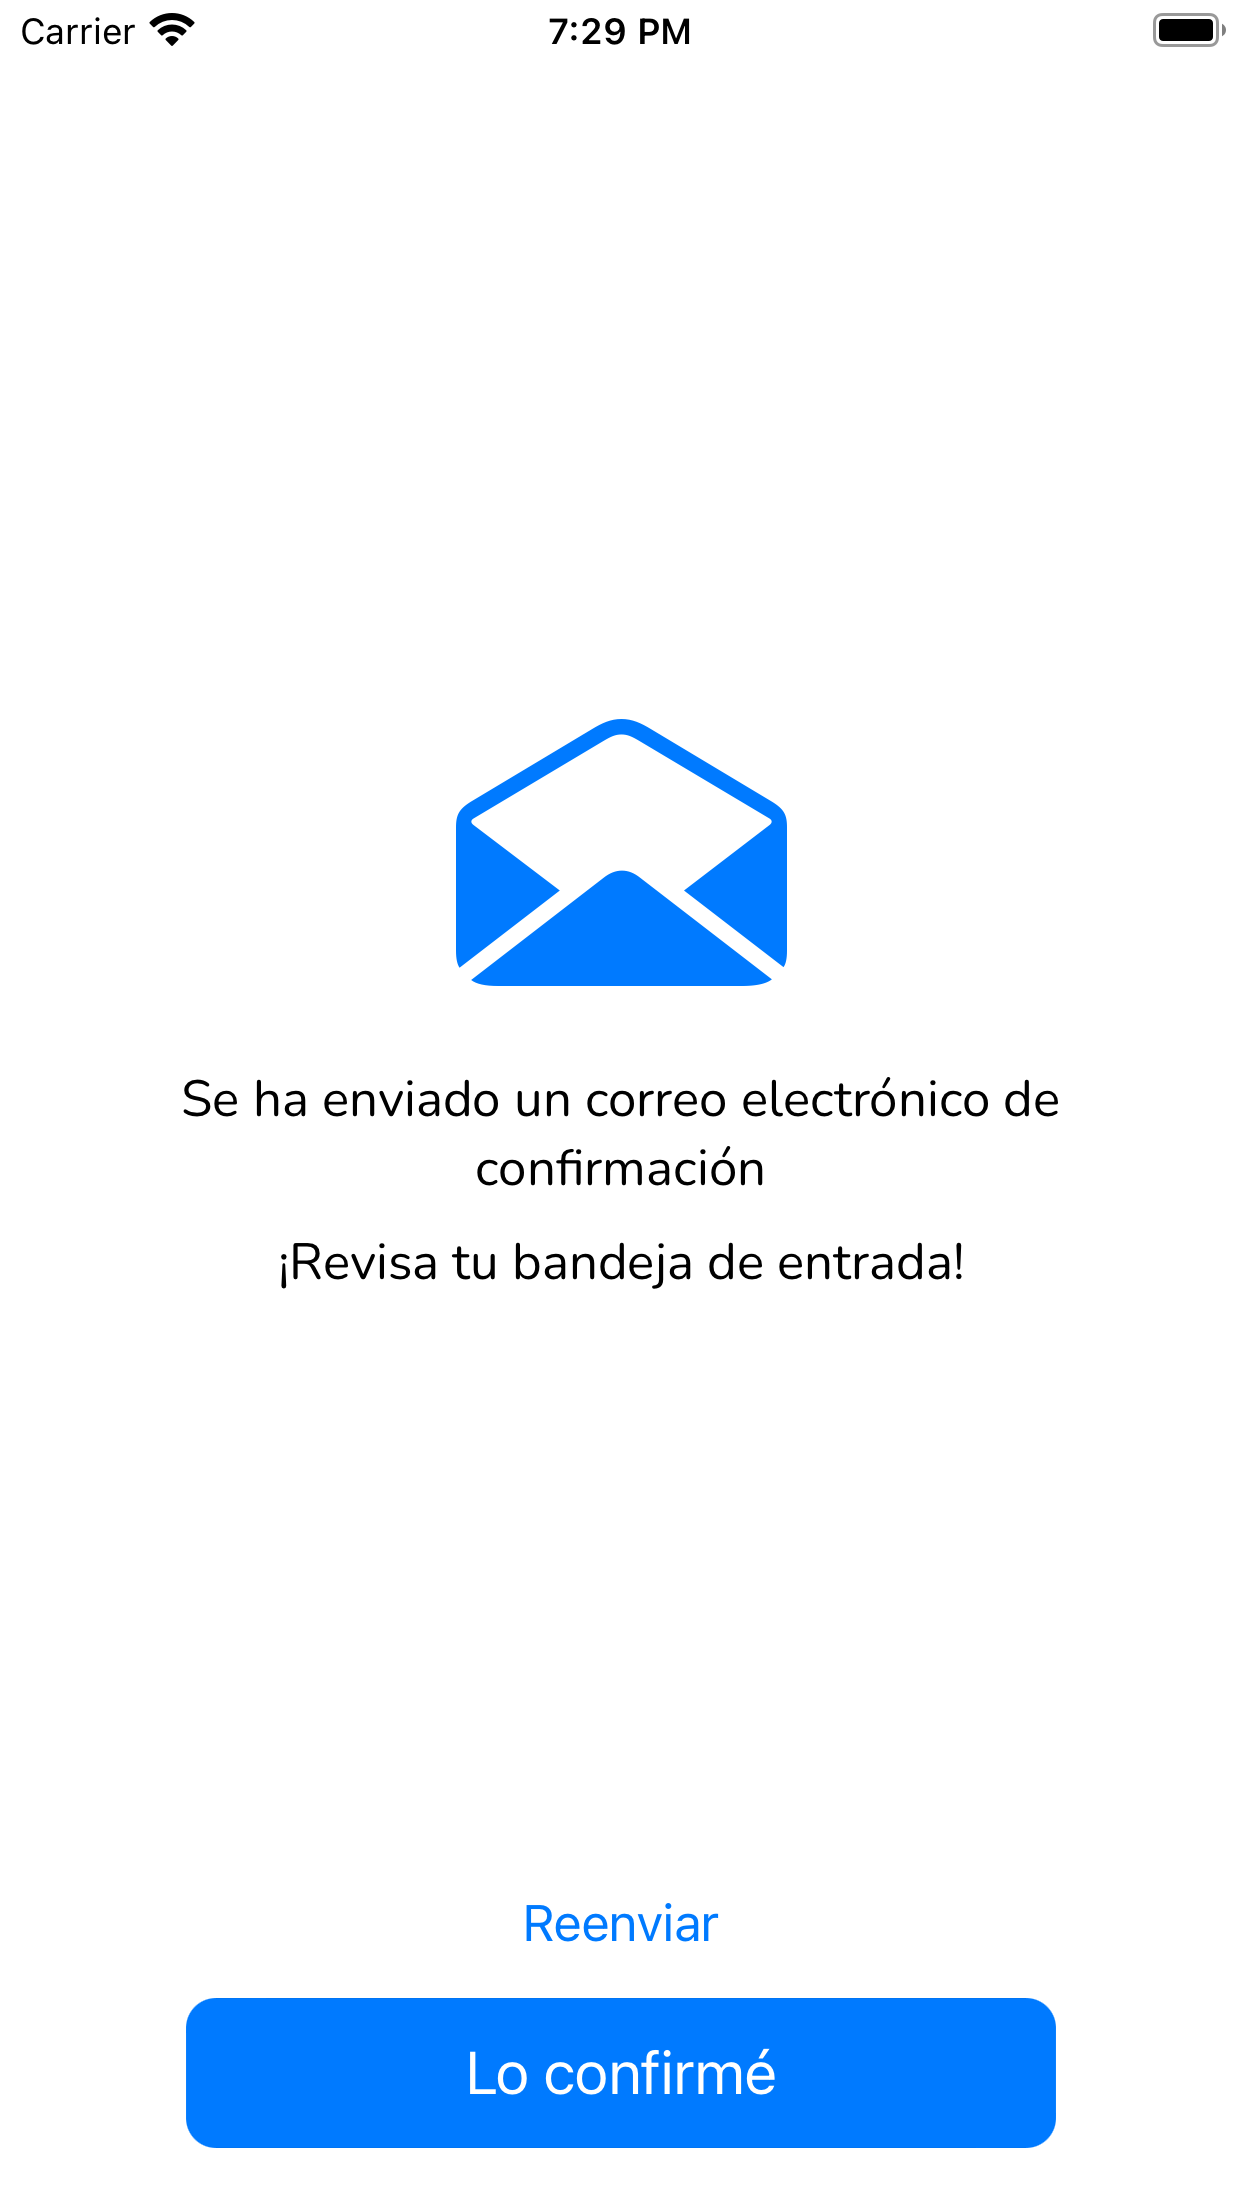
\includegraphics[cframe=black 2pt, width=1\linewidth]{images/manual/registroConfirmacion.png}
    \end{minipage}
    \caption{Login and Register}
    \label{fig:login_register}
\end{figure}

\end{appendices}